\documentclass[ignorenonframetext,]{beamer}
\usetheme{m}
\setbeamertemplate{caption}[numbered]
\setbeamertemplate{caption label separator}{:}
\setbeamercolor{caption name}{fg=normal text.fg}
\setbeamertemplate{bibliography item}{\insertbiblabel}
\setbeamertemplate{bibliography entry title}{}
\setbeamertemplate{bibliography entry location}{}
\setbeamertemplate{bibliography entry note}{}
\usepackage{amssymb,amsmath}
\usepackage{ifxetex,ifluatex}
\usepackage{fixltx2e} % provides \textsubscript
\usepackage{lmodern}
\ifxetex
  \usepackage{fontspec,xltxtra,xunicode}
  \defaultfontfeatures{Mapping=tex-text,Scale=MatchLowercase}
  \newcommand{\euro}{€}
\else
  \ifluatex
    \usepackage{fontspec}
    \defaultfontfeatures{Mapping=tex-text,Scale=MatchLowercase}
    \newcommand{\euro}{€}
  \else
    \usepackage[T1]{fontenc}
    \usepackage[utf8]{inputenc}
      \fi
\fi
% use upquote if available, for straight quotes in verbatim environments
\IfFileExists{upquote.sty}{\usepackage{upquote}}{}
% use microtype if available
\IfFileExists{microtype.sty}{\usepackage{microtype}}{}
\usepackage{longtable,booktabs}
\usepackage{caption}
% These lines are needed to make table captions work with longtable:
\makeatletter
\def\fnum@table{\tablename~\thetable}
\makeatother

% Comment these out if you don't want a slide with just the
% part/section/subsection/subsubsection title:
\AtBeginPart{
  \let\insertpartnumber\relax
  \let\partname\relax
  \frame{\partpage}
}
\AtBeginSection{
  \let\insertsectionnumber\relax
  \let\sectionname\relax
  \frame{\sectionpage}
}
\AtBeginSubsection{
  \let\insertsubsectionnumber\relax
  \let\subsectionname\relax
  \frame{\subsectionpage}
}

\setlength{\parindent}{0pt}
\setlength{\parskip}{6pt plus 2pt minus 1pt}
\setlength{\emergencystretch}{3em}  % prevent overfull lines
\providecommand{\tightlist}{%
  \setlength{\itemsep}{0pt}\setlength{\parskip}{0pt}}
\setcounter{secnumdepth}{0}
\usepackage{stmaryrd}
\usepackage{euler}
\usepackage{pgf}
\usepackage{hyperref}
\usepackage{listings}
\usepackage{bytefield}
\usefonttheme[onlymath]{serif}

\newcommand{\columnsbegin}{\begin{columns}}
\newcommand{\columnsend}{\end{columns}}

\newcommand{\infile}[1]{{\tiny \alert{[#1]}}}
\newcommand{\filelink}[1]{{\alert{#1}}}
\newcommand{\aurl}[1]{\alert{\url{#1}}}
\newcommand{\pandocslide}[2]{\only<#1>{#2}}

\setbeamertemplate{footline}[text line]{%
  {\raisebox{6pt}{\includegraphics[height=0.6cm]{images/galois.pdf}}%
   \hfill%
   \raisebox{6pt}{\it\textcopyright~\number\year~Galois, Inc.  All Rights Reserved.}%
   \hfill%
   \raisebox{6pt}{\insertframenumber/\inserttotalframenumber}
  }
}

\lstset{
  basicstyle=\footnotesize\ttfamily,
  extendedchars=true,
  breaklines=true,
  frame=lrtb,
  showspaces=false,
  showtabs=false,
  %xleftmargin=10pt,
  %xrightmargin=5pt,
  %framexleftmargin=5pt,
  %framexrightmargin=-1pt,
  %framexbottommargin=4pt,
}

\title{Applying Satisfiability to the Analysis~of~Cryptography}
\author{Aaron Tomb, Galois, Inc.}
\date{September 25, 2015}

\begin{document}
\frame{\titlepage}

\begin{frame}{Why Use SAT for Cryptography?}

\begin{itemize}
\tightlist
\item
  Cryptographic algorithms are critical

  \begin{itemize}
  \tightlist
  \item
    Central to commerce, private communication, etc.
  \item
    We want them to be correct
  \end{itemize}
\item
  Cryptography is hard

  \begin{itemize}
  \tightlist
  \item
    Rare expertise
  \item
    Top experts have designed algorithms now known vulnerable
  \item
    Design \(\rightarrow\) implementation can introduce other problems
  \end{itemize}
\item
  Key primitives used in cryptography amenable to SAT

  \begin{itemize}
  \tightlist
  \item
    Can be given denotational semantics in propositional logic
  \item
    Many interesting problems surprisingly tractable
  \end{itemize}
\end{itemize}

\end{frame}

\begin{frame}{Cryptographic Operations as SAT Problems}

\begin{itemize}
\tightlist
\item
  Many primitives naturally made of bit vector operations

  \begin{itemize}
  \tightlist
  \item
    Block ciphers
  \item
    Stream ciphers
  \item
    Hash functions
  \item
    Pseudo-random number generators (PRNGs)
  \end{itemize}
\item
  Public-key algorithms representable, but trickier

  \begin{itemize}
  \tightlist
  \item
    Lots of number theory, including multiplication
  \item
    SMT can alleviate some of this (but tends to be slower on
    bit-vectory things)
  \end{itemize}
\item
  We'll focus on primitives with type
  \(\{0,1\}^{n} \rightarrow \{0,1\}^{m}\)
\end{itemize}

\end{frame}

\begin{frame}[fragile]{Translating Algorithms to Propositional Logic}

\columnsbegin

\column{.4\textwidth}

\begin{itemize}
\tightlist
\item
  A function from the ZUC stream cipher
\end{itemize}

\begin{lstlisting}[language=C,escapechar=@]
uint8_t c = a + b;
if (c & 0x80) {
  c = (c & 0x7F) + 1;
}
return c;
\end{lstlisting}

\column{.6\textwidth}

\pandocslide{1}{\includegraphics[width=\textwidth]{images/expr-1.png}}
\pandocslide{2}{\includegraphics[width=\textwidth]{images/expr-2.png}}
\pandocslide{3}{\includegraphics[width=\textwidth]{images/expr-3.png}}
\pandocslide{4}{\includegraphics[width=\textwidth]{images/expr-4.png}}

\columnsend

\end{frame}

\begin{frame}{Translating Algorithms to Propositional Logic (Cont.)}

\begin{center}
\includegraphics[height=0.8\textheight]{images/addm.pdf}
\end{center}

\end{frame}

\begin{frame}{Specific tools}

\begin{itemize}
\tightlist
\item
  Transalg (Russian Academy of Sciences) \cite{transalg}
\item
  C++ operator overloading (several) \cite{jovanovic2005logical}
\item
  Cryptol and the Software Analysis Workbench (SAW) (Galois)

  \begin{itemize}
  \tightlist
  \item
    Cryptol for describing algorithms concisely
  \item
    SAW for proving properties about them
  \item
    Both freely available!
  \end{itemize}
\end{itemize}

\end{frame}

\begin{frame}{Outline of Examples}

\begin{itemize}
\tightlist
\item
  Each with a concise formula summarizing the SAT problem
\end{itemize}

\begin{center}
$\forall x.~P$ or $\exists y.~Q$
\end{center}

\begin{itemize}
\item
  Cryptol specifications available online
\item
  Analyzed using SAW + ABC
\item
  Cryptol or SAW file names mentioned in slides (e.g. \infile{file.saw})
\end{itemize}

\begin{center}
\aurl{https://github.com/galoisinc/sat2015-crypto}
\end{center}

\begin{center}
\filelink{file.saw} $\rightarrow$ \filelink{examples/file.saw}
\end{center}

\end{frame}

\begin{frame}{Pseudo-Random Generators}

\begin{itemize}
\tightlist
\item
  Randomness is critical to cryptography

  \begin{itemize}
  \tightlist
  \item
    Keys must be unpredictable, or they're vulnerable
  \end{itemize}
\item
  Typical structure:

  \begin{center}
  seed $\rightarrow$ pseudo-random function $\rightarrow$ pseudo-random value
  \end{center}
\item
  Seed often comes from ``true'' random source
\item
  But it's critical not to lose entropy from this source!
\end{itemize}

\end{frame}

\begin{frame}{Injectivity of PRNG Seeding}

\begin{itemize}
\tightlist
\item
  Bug in Android cryptographic PRNG discarded entropy
\item
  Intended: 160 bits of entropy, from system PRNG to SHA-1
  \includegraphics[width=0.95\textwidth]{images/prng-intended.pdf}
\item
  Implemented: 64 bits of entropy survive
  \includegraphics[width=0.95\textwidth]{images/prng-buggy.pdf}
\item
  Used to steal around \$6k of BitCoin
\item
  Fixed in Android 4.4 (KitKat)
\item
  Similar weaknesses existed in Debian, FreeBSD at times
\end{itemize}

\end{frame}

\begin{frame}{Injectivity of PRNG Seeding (cont.)}

\begin{center}
$\forall x, y.~x \neq y \Rightarrow f(x) \neq f(y)$
\end{center}

\begin{itemize}
\tightlist
\item
  Here, \(x\) and \(y\) come from system PRNG, \(f\) is code between
  system PRNG and SHA-1
\item
  Easily provable with SAT solver \infile{android-prng.saw}

  \begin{itemize}
  \tightlist
  \item
    Symbolic execution: Java code \(\rightarrow\) AIG
  \item
    Annotation on system RNG variables, input to SHA-1
  \item
    ABC can find collision (0.017s), prove fixed version (0.010s)
  \end{itemize}
\item Dörre and Klebanov used a different approach to prove the fixed code
  injective \cite{dorre2015prng}

  \begin{itemize}
  \tightlist
  \item
    Information flow annotations on methods using a contract
    verification tool (KeY) and 95 manual proof steps
  \end{itemize}
\end{itemize}

\end{frame}

\begin{frame}{Hash Functions}

\begin{center}
\includegraphics[width=\textwidth]{images/Merkle-damgard.pdf}
\end{center}

\begin{itemize}
\tightlist
\item
  Key property: hard to find two messages that have the same hash (a
  \alert{collision})
\item
  Often built using Merkle--Damgård construction, iterating compression
  function
\item
  Compression function \(f\) usually \(n\) iterations of simpler
  function \(g\)
\end{itemize}

\end{frame}

\begin{frame}{Hash Collisions and Inversion}

\begin{center}
$\exists x, y.~x \neq y \wedge f(x) = f(y)$
\end{center}

\begin{itemize}
\tightlist
\item
  Discovering a collision
\item
  Black box search in \(O(2^{n/2})\)
\end{itemize}

\begin{center}
$\exists x.~f(x) = a$ (for some known value $a$)
\end{center}

\begin{itemize}
\item
  Discovering message given hash value (inversion)
\item
  Harder than finding a collision (\(O(2^{n})\))
\item
  We want to know that it's \alert{hard} to solve these problems
\end{itemize}

\end{frame}

\begin{frame}{Finding Hash Collisions}

\begin{itemize}
\tightlist
\item Mironov and Zhang analyzed collisions in MD4, MD5, and SHA-0
  \cite{mironov2006hash}

  \begin{itemize}
  \tightlist
  \item
    Direct translation of MD4 \(\rightarrow\) \(2^{22}\) solutions in
    \(<\) 1h
  \item
    Collision on full MD5 in around 100h

    \begin{itemize}
    \tightlist
    \item
      Reduced rounds much easier (25 in 38s with ABC) \infile{MD5.saw}
    \item
      Used differential path derived manually (more on this later)
    \end{itemize}
  \item
    Estimated around 3 million (2006-era) CPU hours for SHA-0
  \end{itemize}
\item
  No known collisions on SHA-1 from this, but it may be a matter of time

  \begin{itemize}
  \tightlist
  \item
    Algorithm (not SAT-based) to find collisions in \(2^{63}\)
    operations
  \end{itemize}
\end{itemize}

\end{frame}

\begin{frame}{Evaluating SHA-3 Candidates}

\begin{itemize}
\tightlist
\item
  Many candidate algorithms for the SHA-3 standard
\item
  No preimages discoverable by SAT on full algorithms
\item
  Homsirikamol et al. found preimages for fewer rounds \cite{homsirikamol2012sha3}

  \begin{itemize}
  \tightlist
  \item
    Direct translation, with no manual cryptanalysis
  \end{itemize}
\end{itemize}

\begin{longtable}[c]{@{}llll@{}}
\toprule
Algorithm & Rounds & Security margin & Code\tabularnewline
\midrule
\endhead
SHA-1 & 21 & 74\% (21/80) & \filelink{SHA-0-1.saw} (36s)\tabularnewline
SHA-256 & 16 & 75\% (16/64) & \filelink{SHA265.saw}
(1.3s)\tabularnewline
Keccak-256 & 2 & 92\% (2/24) & N/A\tabularnewline
BLAKE-256 & 1 & 93\% (1/14) & \filelink{Blake256.saw}
(17s)\tabularnewline
Groestl-256 & 0.5 & 95\% (0.5/10) & N/A\tabularnewline
JH-256 & 2 & 96\% (2/42) & N/A\tabularnewline
Skein-512-256 & 1 & 99\% (1/72) & N/A\tabularnewline
\bottomrule
\end{longtable}

\end{frame}

\begin{frame}{Block Ciphers}

\columnsbegin

\column{.5\textwidth}

\begin{itemize}
\tightlist
\item
  Given a key, a block cipher is a pseudo-random permutation

  \begin{itemize}
  \tightlist
  \item
    Therefore, invertible (for a fixed key)
  \end{itemize}
\item
  Often built as a substitution-permutation network

  \begin{itemize}
  \tightlist
  \item
    Will return to S-boxes
  \end{itemize}
\end{itemize}

\column{.5\textwidth}

\includegraphics[width=\textwidth]{images/spn2.png}

\columnsend

\end{frame}

\begin{frame}{Key Expansion}

\columnsbegin

\column{.4\textwidth}

\begin{center}
\includegraphics[height=0.8\textheight]{images/DES-key-schedule.png}
\end{center}

\column{.6\textwidth}

\begin{itemize}
\tightlist
\item
  Symmetric encryption often involves a single shared key

  \begin{itemize}
  \tightlist
  \item
    Block ciphers typically need one key per round
  \item
    Stream ciphers need one ``key'' per message block
  \end{itemize}
\item
  So we need to \alert{expand} the initial key in an unpredictable way
\item
  Should preserve size of key space
\end{itemize}

\columnsend

\end{frame}

\begin{frame}{Injectivity of Key Expansion}

\begin{center}
$\forall x, y.~x \neq y \Rightarrow f(x) \neq f(y)$
\end{center}

\begin{itemize}
\tightlist
\item
  Provable injectivity of SIMON, Salsa20 key expansion

  \begin{itemize}
  \tightlist
  \item
    Around 10-20s with ABC \infile{simon.saw} \infile{Salsa20.saw}
  \end{itemize}
\item
  Provable injectivity of AES key expansion

  \begin{itemize}
  \tightlist
  \item
    A little under a minute with ABC \infile{AES.saw}
  \end{itemize}
\item
  ZUC, a stream cipher for GSM, had a vulnerability

  \begin{itemize}
  \tightlist
  \item
    Key expansion not injective in ZUC 1.4 (0.5s) \infile{zuc.saw}
  \item
    Provably fixed in ZUC 1.5 (0.6s) \infile{zuc.saw}
  \item Originally shown with custom search procedure taking 3m
    \cite{wang2012zuc}
  \end{itemize}
\item
  \alert{Not injective} for DES!

  \begin{itemize}
  \tightlist
  \item
    Known to have weak keys
  \item
    Can show quickly with ABC (0.08s) \infile{DES.saw}
  \end{itemize}
\end{itemize}

\end{frame}

\begin{frame}{Encryption \(\rightarrow\) Decryption}

\begin{center}
$\exists m.~E(m, k) = c$ for known $k$ and $c$
\end{center}

\begin{itemize}
\tightlist
\item
  Decrypting using encryption code
\item
  This actually works!

  \begin{itemize}
  \tightlist
  \item
    Relatively efficient for DES (0.2s), 3DES (0.8s) \infile{DES.saw}
    \infile{3DES.saw}
  \item
    More modern ciphers slower:

    \begin{itemize}
    \tightlist
    \item
      AES (1.5m) \infile{AES.saw}
    \item
      SIMON (3.6m) \infile{simon.saw}
    \item
      Speck (20s) \infile{speck.saw}
    \end{itemize}
  \end{itemize}
\item
  Can also run the encryption directly:

  \begin{itemize}
  \tightlist
  \item
    \(\exists c.~E(m, k) = c\) for known \(m\) and \(k\)
  \item
    Usually takes 1/5 to 1/2 the time of decryption
  \item
    Not really useful, but illustrates the flexibility of SAT
  \end{itemize}
\end{itemize}

\end{frame}

\begin{frame}{Block Cipher Consistency}

\begin{center}
$\forall m, k.~D(E(m, k), k) = m$
\end{center}

\begin{itemize}
\tightlist
\item
  For a block cipher with encryption function \(E\), decryption \(D\)
\item
  Feasible to show for many ciphers

  \begin{itemize}
  \tightlist
  \item
    DES (4s) \infile{DES.saw}
  \item
    3DES (8s) \infile {3DES.saw}
  \item
    SIMON (6.2m) \infile{simon.saw}
  \item
    Speck (2.7m) \infile{speck.saw}
  \end{itemize}
\item
  Hard to show for AES (at least with encodings and solvers we've tried)
  \infile{AES.saw}
\end{itemize}

\end{frame}

\begin{frame}{Equivalence Checking}

\begin{center}
$\forall x.~f(x) = g(x)$
\end{center}

\begin{itemize}
\tightlist
\item
  Two functions give equivalent output for all inputs
\item
  AIGs give distinct benefits over direct CNF creation

  \begin{itemize}
  \tightlist
  \item
    Intuitive construction
  \item
    Sharing subterms reduces overall expression size
  \item
    SAT sweeping helps identify candidate equivalences

    \begin{itemize}
    \tightlist
    \item
      Especially effective for cryptography
    \end{itemize}
  \item
    Use best available SAT solver for final phase
  \end{itemize}
\item Works on many core cryptographic primitives, including AES (on a single
  block) (\textasciitilde{}6.4m) \infile{AES-eq.saw}
\end{itemize}

\end{frame}

\begin{frame}{Equivalence Checking Illustrated}

\pandocslide{1}{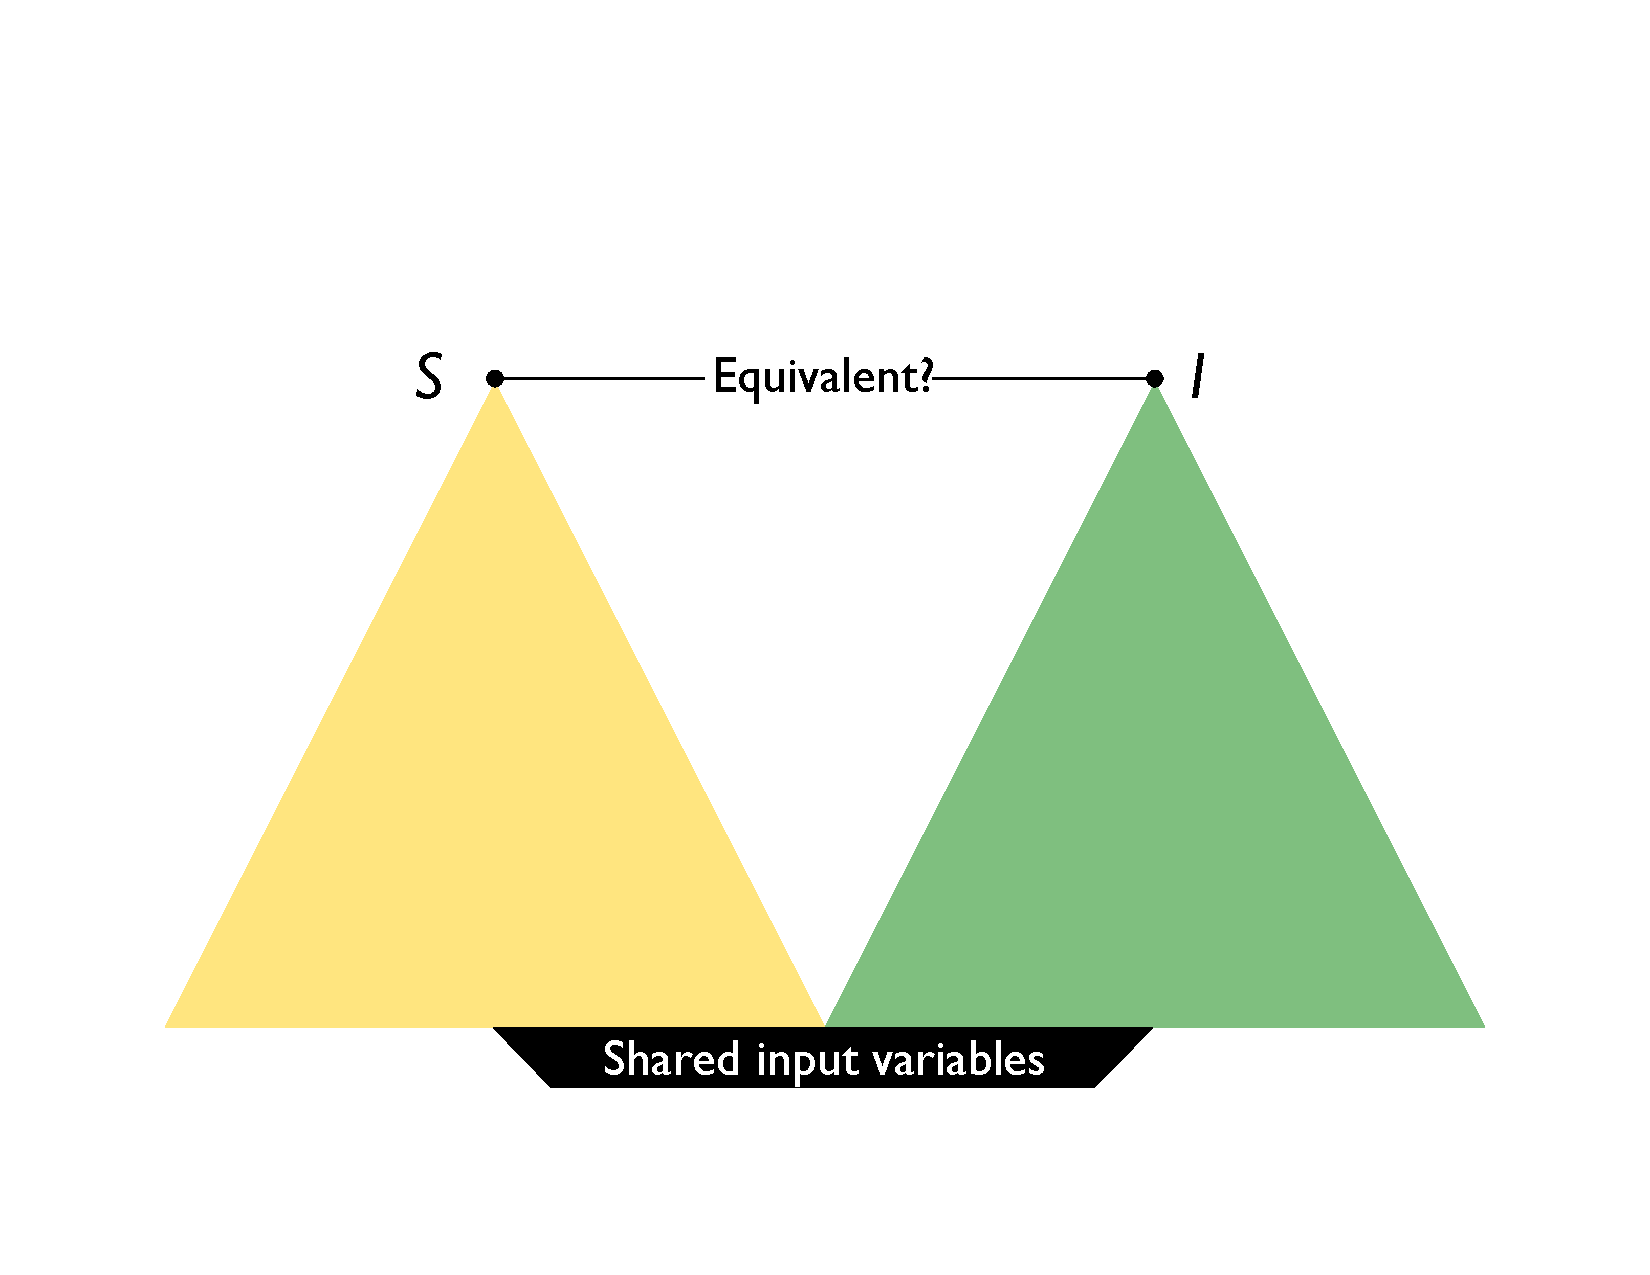
\includegraphics[height=0.9\textheight]{images/Block1.pdf}}
\pandocslide{2}{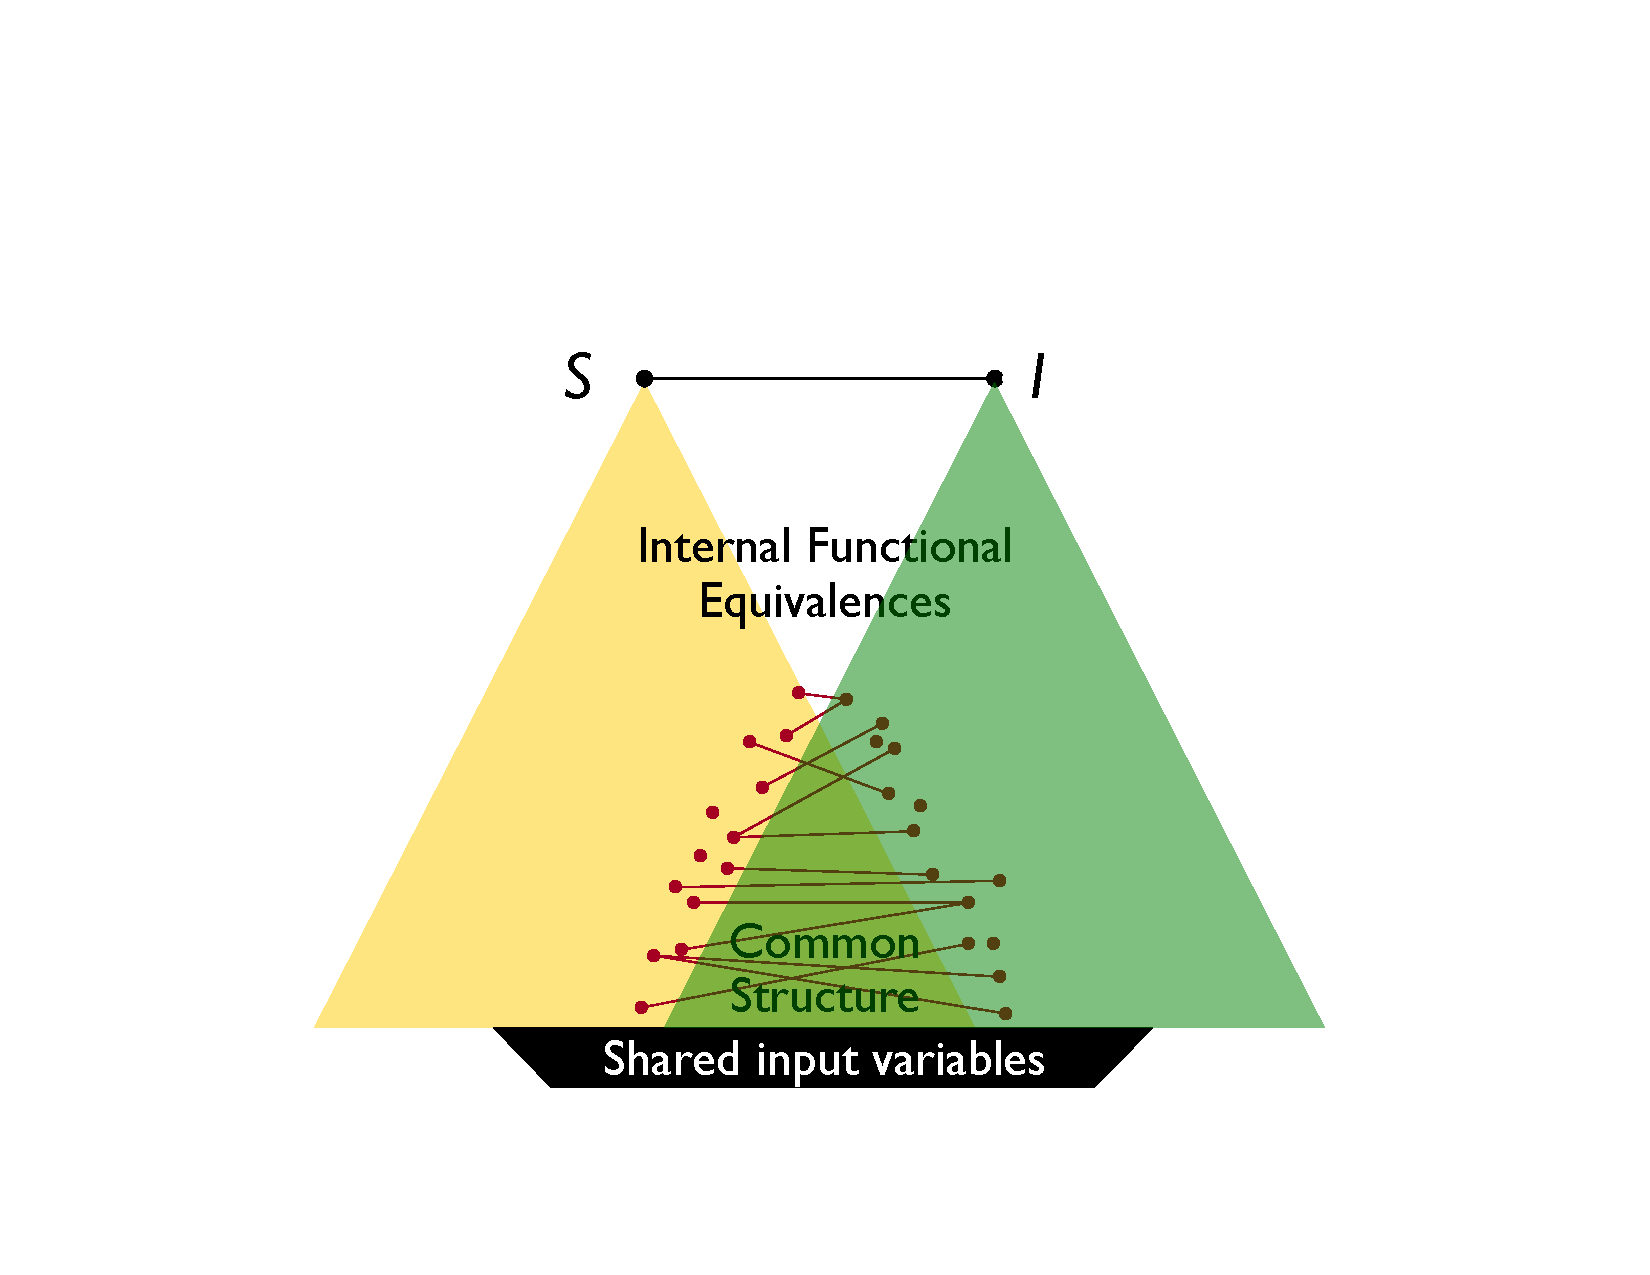
\includegraphics[height=0.9\textheight]{images/Block2.pdf}}
\pandocslide{3}{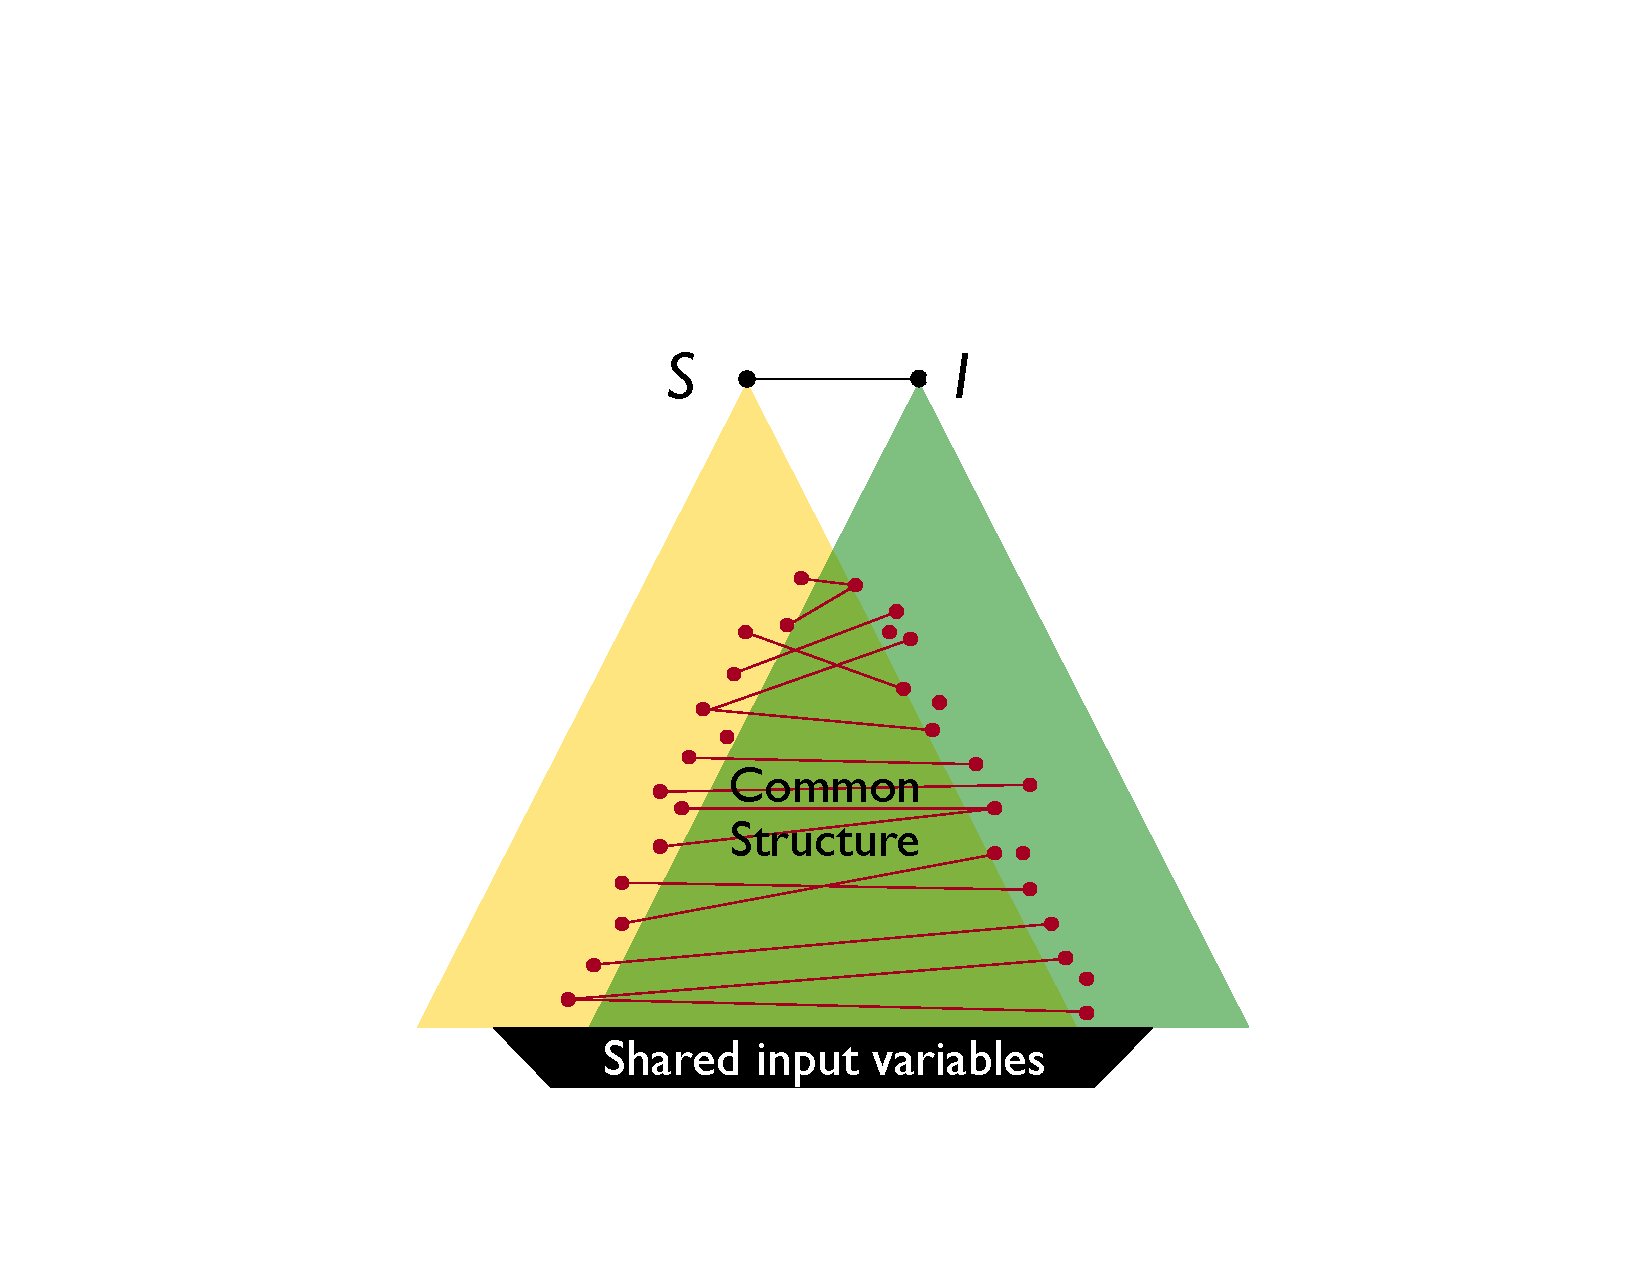
\includegraphics[height=0.9\textheight]{images/Block3.pdf}}
\pandocslide{4}{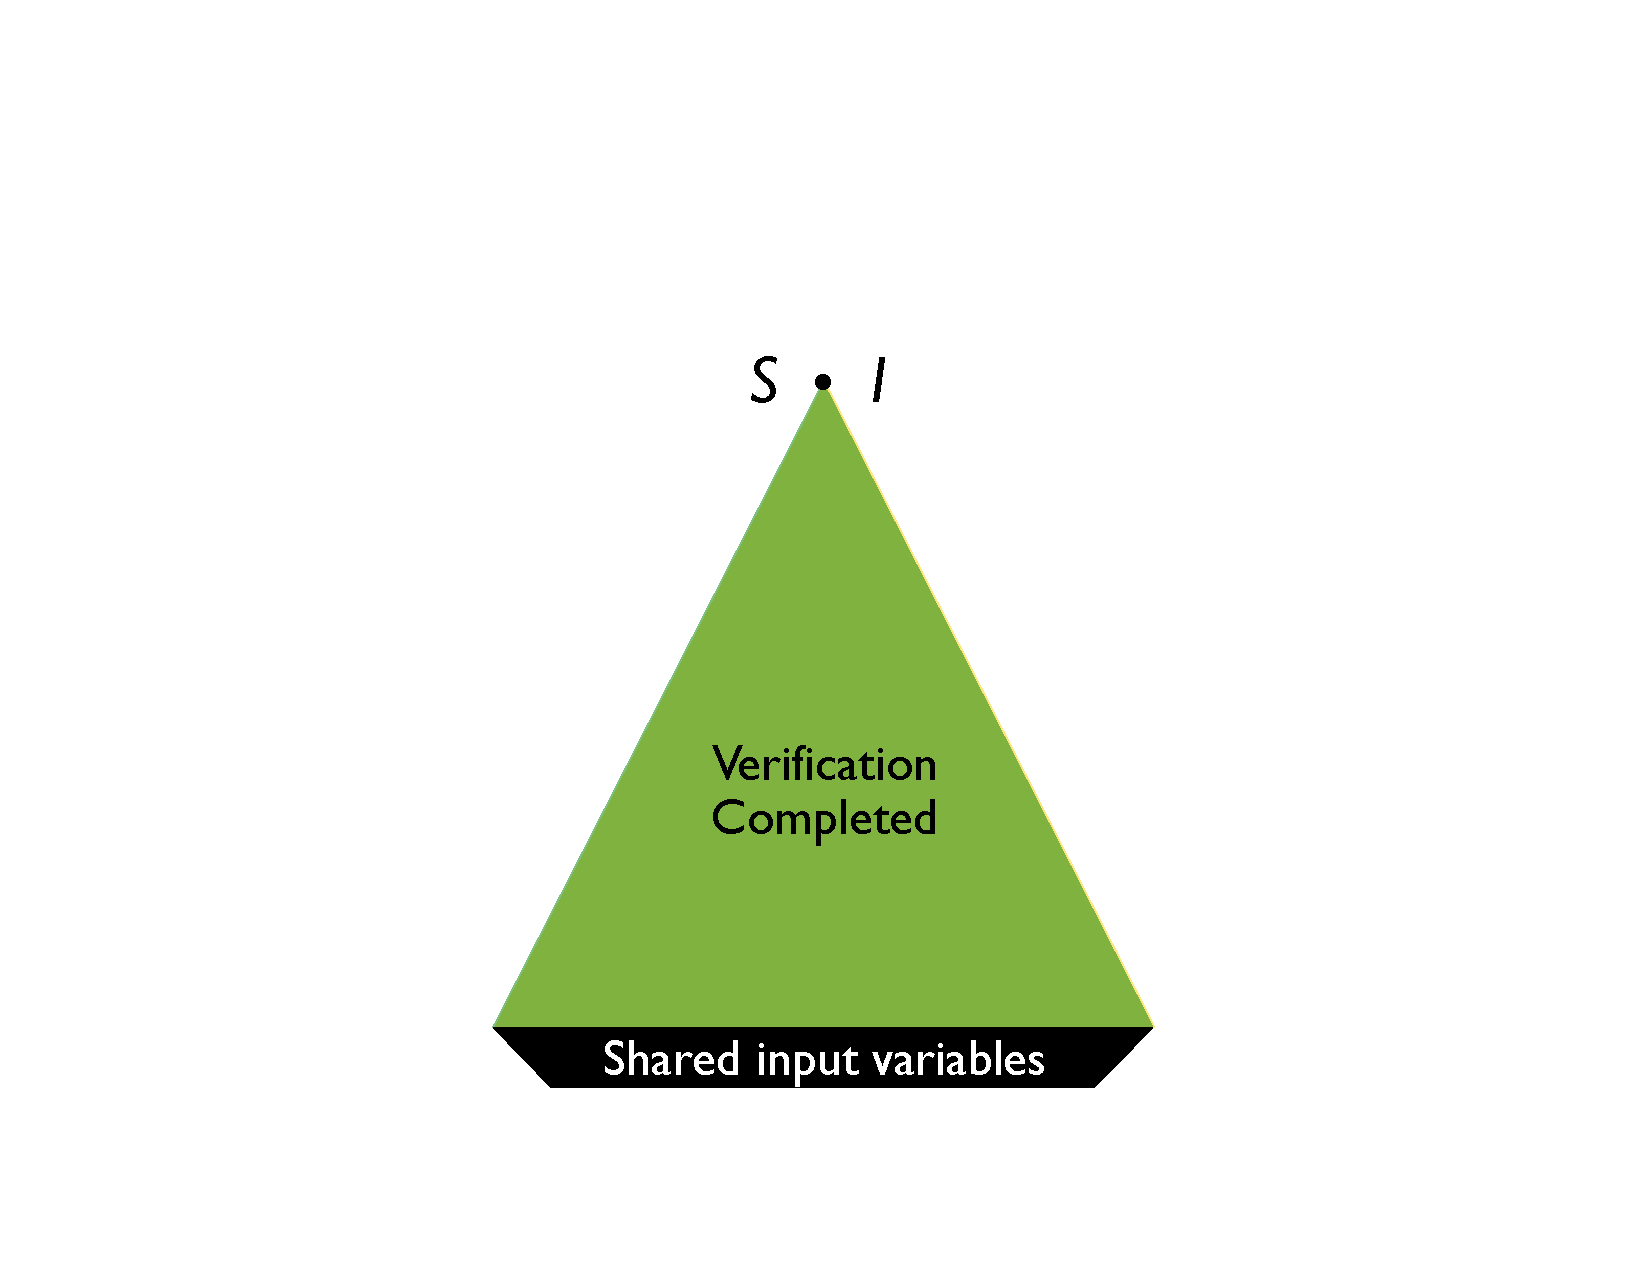
\includegraphics[height=0.9\textheight]{images/Block4.pdf}}

\end{frame}

\begin{frame}{Compositional Equivalence Checking: Motivation}

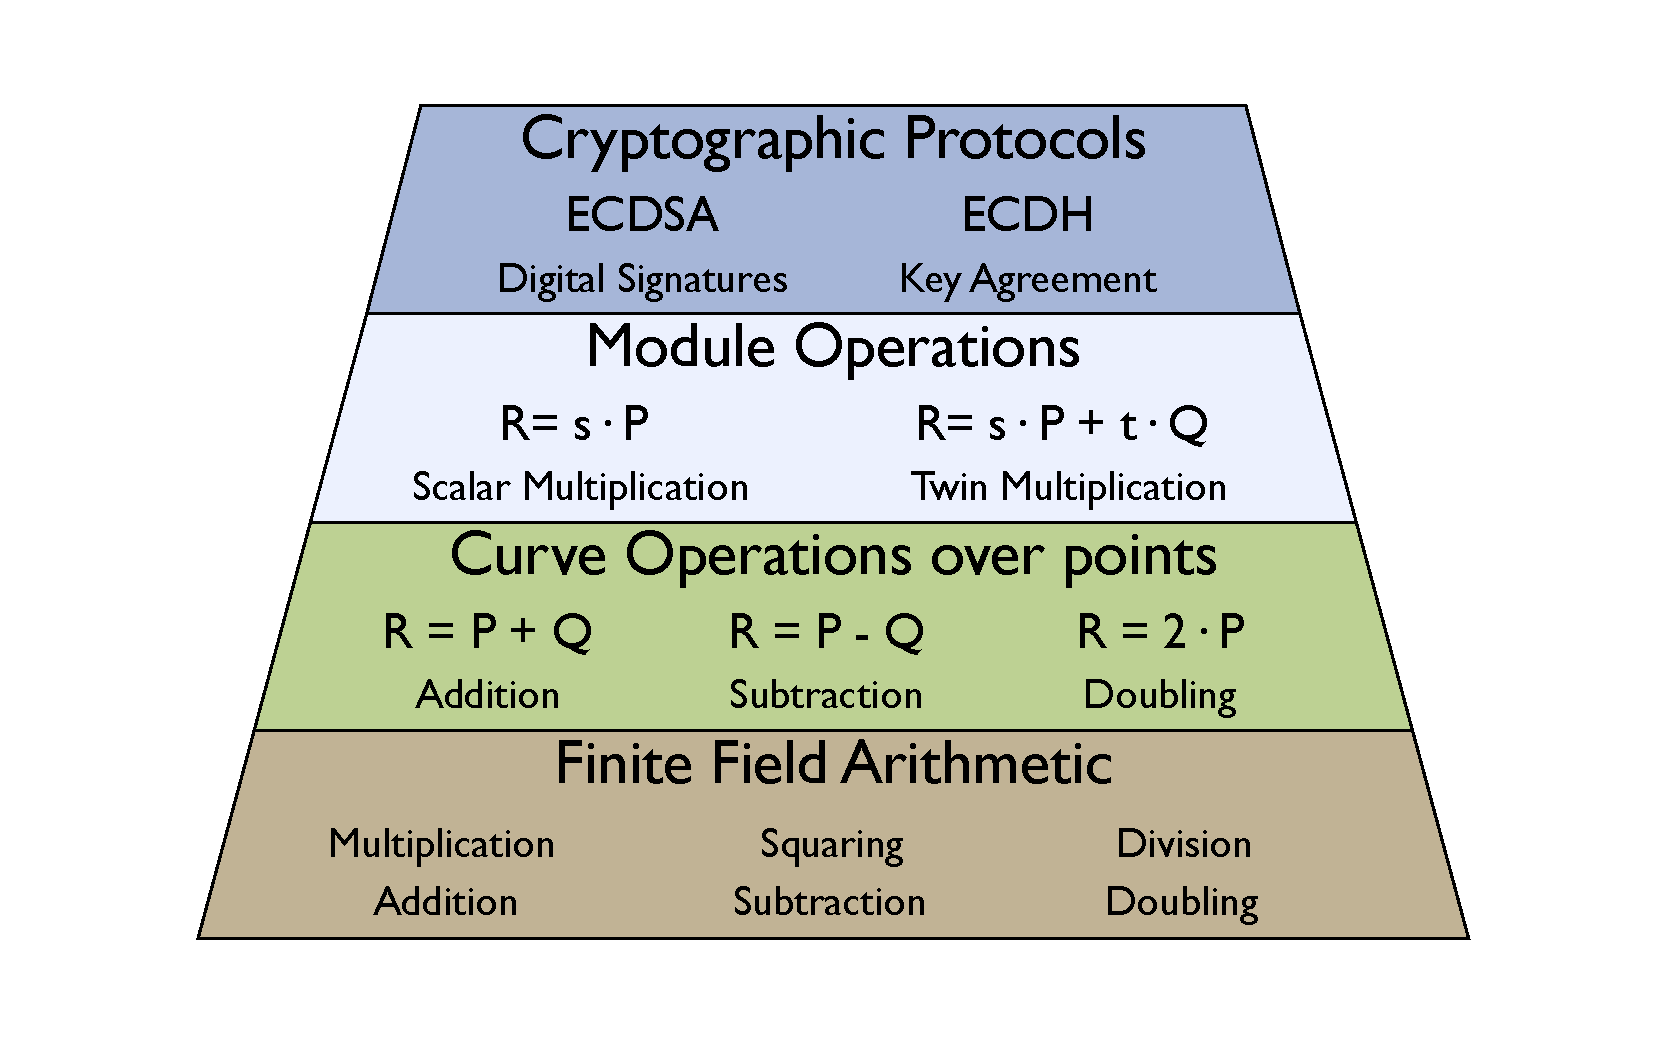
\includegraphics[width=\textwidth]{images/ECC.pdf}

\end{frame}

\begin{frame}{Compositional Equivalence Checking}

\begin{itemize}
\tightlist
\item
  Key tool: uninterpreted functions
\item
  Symbolic execution turns imperative code into functional code

  \begin{itemize}
  \tightlist
  \item
    So procedure calls can be uninterpreted functions
  \item
    \alert{If} we know all inputs and outputs
  \end{itemize}
\item Used for checking equivalence between Cryptol and Java ECDSA
  implementations

  \begin{itemize}
  \tightlist
  \item
    Takes around 5 minutes to run
  \item Takes \textasciitilde{}1500 lines of script (mostly I/O mapping, rewrite
    rules)
  \item
    ABC for leaves, rewriting + Z3 for higher layers
  \end{itemize}
\end{itemize}

\end{frame}

\begin{frame}{Linear Cryptanalysis}

\begin{itemize}
\tightlist
\item
  Attack on symmetric block ciphers
\item
  Known plaintext attack: assumes attacker has some set of \((m, c)\)
  pairs
\item
  Basic idea: can we approximate the encryption function by a linear
  function?

  \begin{itemize}
  \tightlist
  \item
    Where \emph{linear} here means made up entirely of XOR operations
  \end{itemize}
\item
  Any time the encryption function agrees with a linear function too
  often, this can ease cryptanalysis
\item
  Can use \#SAT to count how often it behaves linearly
\end{itemize}

\end{frame}

\begin{frame}{Differential Cryptanalysis}

\begin{itemize}
\tightlist
\item
  Like linear cryptanalysis, known plaintext attack on symmetric block
  ciphers
\item
  Analysis of how differences in input affect differences in output
\item
  Disproportional effects can be exploitable
\item
  A \alert{differential characteristic} is a set of differences as they
  traverse a path through the algorithm
\item
  Can use \#SAT to calculate the distributions of differential
  characteristics
\end{itemize}

\end{frame}

\begin{frame}{Cryptanalysis of SIMON}

\begin{itemize}
\tightlist
\item
  SIMON is a lightweight block cipher published recently
\item
  Kölbl \emph{et al.} used SAT for linear and differential cryptanalysis of
  SIMON \cite{kolbl2015simon} \infile{simon-diff.saw}
\item
  Using \#SAT to calculate differential characteristic distributions
\item
  Not direct analysis of code, but of manually-derived simplification
\item
  Serves as an additional tool for cryptanalysis, not push-button
\item
  Suggests slightly different parameters possibly preferable to
  published numbers
\end{itemize}

\end{frame}

\begin{frame}{Side Channel Analysis}

\begin{center}
\includegraphics[width=0.9\textwidth]{images/sidechannel.jpg}
\end{center}

\begin{itemize}
\tightlist
\item
  Traditional side channel analysis

  \begin{itemize}
  \tightlist
  \item
    Observe specific part of last round of block cipher
  \item
    Combine with pre-calculated formulas to recover key
  \end{itemize}
\item
  Caveat: only works if you can observe the right signals
\end{itemize}

\end{frame}

\begin{frame}{Using SAT for Side Channel Analysis}

\begin{itemize}
\tightlist
\item
  Example: hardware implementation

  \begin{itemize}
  \tightlist
  \item
    Encode entire algorithm (as implemented) as a boolean circuit
  \item
    Observe any internal values possible
  \item
    Constrain internal variables accordingly
  \item
    Try to solve for key (or other aspects of state)
  \end{itemize}
\item
  More information than just inputs or outputs
\item
  Can use \alert{any internal variable} in the algorithm
\item
  Hamming weights plus a handful of \((m, c)\) pairs enough to recover
  AES key \cite{mohamed2012improved-sc}
\end{itemize}

\end{frame}

\begin{frame}{Creating Code: Optimal S-Boxes}

\begin{itemize}
\tightlist
\item
  S-boxes intended to unpredictably substitute bits

  \begin{itemize}
  \tightlist
  \item
    Ideally indistinguishable from a random function
  \item
    But in practice representable as a short program using only linear
    operations
  \end{itemize}
\item
  Generating optimal S-boxes:

  \begin{itemize}
  \tightlist
  \item
    Or any function on a small domain
  \item
    \(\exists p.~\llbracket{}p\rrbracket{}(x_{0}) = y_{0} \wedge \dots \wedge  \llbracket{}p\rrbracket{}(x_{n}) = y_{n}\)
  \end{itemize}
\item
  Fuhs \emph{et al.} found a 23-instruction AES S-box program
  \cite{fuhs2010sbox}

  \begin{itemize}
  \tightlist
  \item
    Less than a minute with MiniSat
  \item
    Proving unsatisfiability of 22 instructions took 106 hours
    (CryptoMiniSat)
  \end{itemize}
\end{itemize}

\end{frame}

\begin{frame}{Creating Code: General Synthesis}

\begin{itemize}
\tightlist
\item
  General synthesis:

  \begin{itemize}
  \tightlist
  \item
    \(\exists p.~\forall x.~\llbracket{}p\rrbracket{}(x) = f(x)\)
  \end{itemize}
\item
  Generating efficient implementations:

  \begin{itemize}
  \tightlist
  \item
    \(\min p.~\forall x.~\llbracket{}p\rrbracket{}(x) = f(x)\)
  \end{itemize}
\item
  Generally, a hard problem

  \begin{itemize}
  \tightlist
  \item
    But QBF solvers are getting powerful
  \item
    Many papers in SMT community about this problem recently
  \end{itemize}
\end{itemize}

\end{frame}

\begin{frame}{Other Examples}

\begin{itemize}
\item
  Cryptographic protocol analysis
\item
  Diffusion analysis
\item
  Differential fault analysis
\item
  Constructing new encryption schemes
\item
  What's next?
\end{itemize}

\end{frame}

\begin{frame}{Currently Difficult Problems}

\begin{itemize}
\tightlist
\item
  Some problems are difficult with current solvers, but potentially
  tractable

  \begin{itemize}
  \tightlist
  \item
    AES equivalence in CNF (tractable using SAT sweeping!)
  \item
    AES consistency
  \item
    Good benchmarks for solver improvement!
  \end{itemize}
\item
  Some problems that are intrinsically difficult (we hope)

  \begin{itemize}
  \tightlist
  \item
    Multiplication difficulty seems related to hardness of factoring
  \item
    Finding a hash collisions had better be hard
  \item
    Finding \(k\) given \(m\), \(c\) should be hard, too
  \end{itemize}
\item
  Synthesis is currently hard

  \begin{itemize}
  \tightlist
  \item
    But provers are getting better at this (QBF and
    \(\exists\forall\)-SMT)
  \end{itemize}
\item
  Very similar problems can be different in difficulty

  \begin{itemize}
  \tightlist
  \item
    Reversing AES vs.~finding \(k\) from \(m\), \(c\)
  \end{itemize}
\end{itemize}

\end{frame}

\begin{frame}{Tools}

\begin{itemize}
\tightlist
\item
  Cryptol is a DSL for cryptographic code

  \begin{itemize}
  \tightlist
  \item
    Allows expression of algorithms at a high-level of abstraction
  \item
    Built-in connection to SMT solvers
  \item
    BSD-licensed

    \begin{itemize}
    \tightlist
    \item
      \aurl{http://cryptol.net}
    \end{itemize}
  \end{itemize}
\item
  The Software Analysis Workbench (SAW) allows analysis of
  implementations

  \begin{itemize}
  \tightlist
  \item
    Symbolic execution of Cryptol, C, Java
  \item
    Bindings to SMT and SAT solvers, including ABC
  \item
    Freely available (with source) for non-commercial use

    \begin{itemize}
    \tightlist
    \item
      \aurl{http://saw.galois.com}
    \end{itemize}
  \end{itemize}
\item
  All the examples from this talk are available

  \begin{itemize}
  \tightlist
  \item
    \aurl{https://github.com/galoisinc/sat2015-crypto}
  \end{itemize}
\end{itemize}

\end{frame}

\begin{frame}{Summing it up}

\begin{itemize}
\tightlist
\item
  Cryptography and SAT go very nicely together

  \begin{itemize}
  \tightlist
  \item
    Easily representable as propositional formulas
  \item
    AIGs are super handy! (not just for hardware)
  \end{itemize}
\item
  More use of SAT during algorithm development will make our crypto
  stronger

  \begin{itemize}
  \tightlist
  \item
    And it's happening: see SHA-3, Trivium, SIMON, etc.
  \end{itemize}
\item
  Nice source of hard benchmark problems for solvers
\end{itemize}

\begin{center}
\aurl{https://github.com/galoisinc/sat2015-crypto}
\end{center}

\end{frame}

\begin{frame}[allowframebreaks]{References}
  \bibliographystyle{plain}
  \bibliography{talk}
\end{frame}

\end{document}
